\chapter{Methodology}%
\label{chapter:methodology}



Unity 3D engine will allow robot model development, enabling detailed and interactive digital twins with bilateral communication capabilities. By utilizing Vuforia for precise pose registration, the system ensures accurate spatial alignment between the virtual and physical robots.

To enhance user awareness and prevent accidents, the system will implement visual and audio cues within the \ac{AR} environment, including safety-zone interactions and audio alerts. These features provide intuitive feedback to users, improving situational awareness during human--robot collaboration. The robot manipulation interface will be designed to be user-friendly, allowing non-expert users to operate the robot remotely using a handheld device (\ac{HHD}). This accessibility ensures that a wider range of users can effectively interact with the robotic system without extensive training.

Real-time updates of the robot's position and workspace visualization will be provided through camera feed transmission, offering remote users a comprehensive view of the operational environment. This feature addresses the limitations identified in existing literature, where remote users often lack sufficient context and visibility of the workspace.

% Furthermore, the proposed system will address challenges identified in the state-of-the-art review, such as networking latency and positioning accuracy. By implementing optimized communication protocols and advanced tracking algorithms, the system aims to ensure efficient and safe human--robot collaboration. These improvements will not only enhance the performance of the system but also contribute valuable insights to the field, bridging the gap between on-site and remote interaction capabilities in industrial applications.

Overall, this project seeks to expand upon current research by providing a holistic solution that integrates advanced technologies to facilitate seamless collaboration between humans and robots, regardless of physical location. By focusing on both on-site and remote users, the system aims to enhance flexibility, safety, and efficiency in various industrial scenarios.




Initially, Unity software was used in order to develop an application that enabled the on-site member to interact with the robot by utilizing 
virtual and augmented reality to its favor.  

% The developed work, so far, will be explained in this chapter.

In order to start addressing the mentioned challenges, a first effort has been made. A robotic arm, UR10e, from Universal Robots, 
available at IRIS LAB \ref{f:ur10e_iris}, was used as a dynamic agent to assist in shared activities.

\begin{figure}[h]
    \centering
    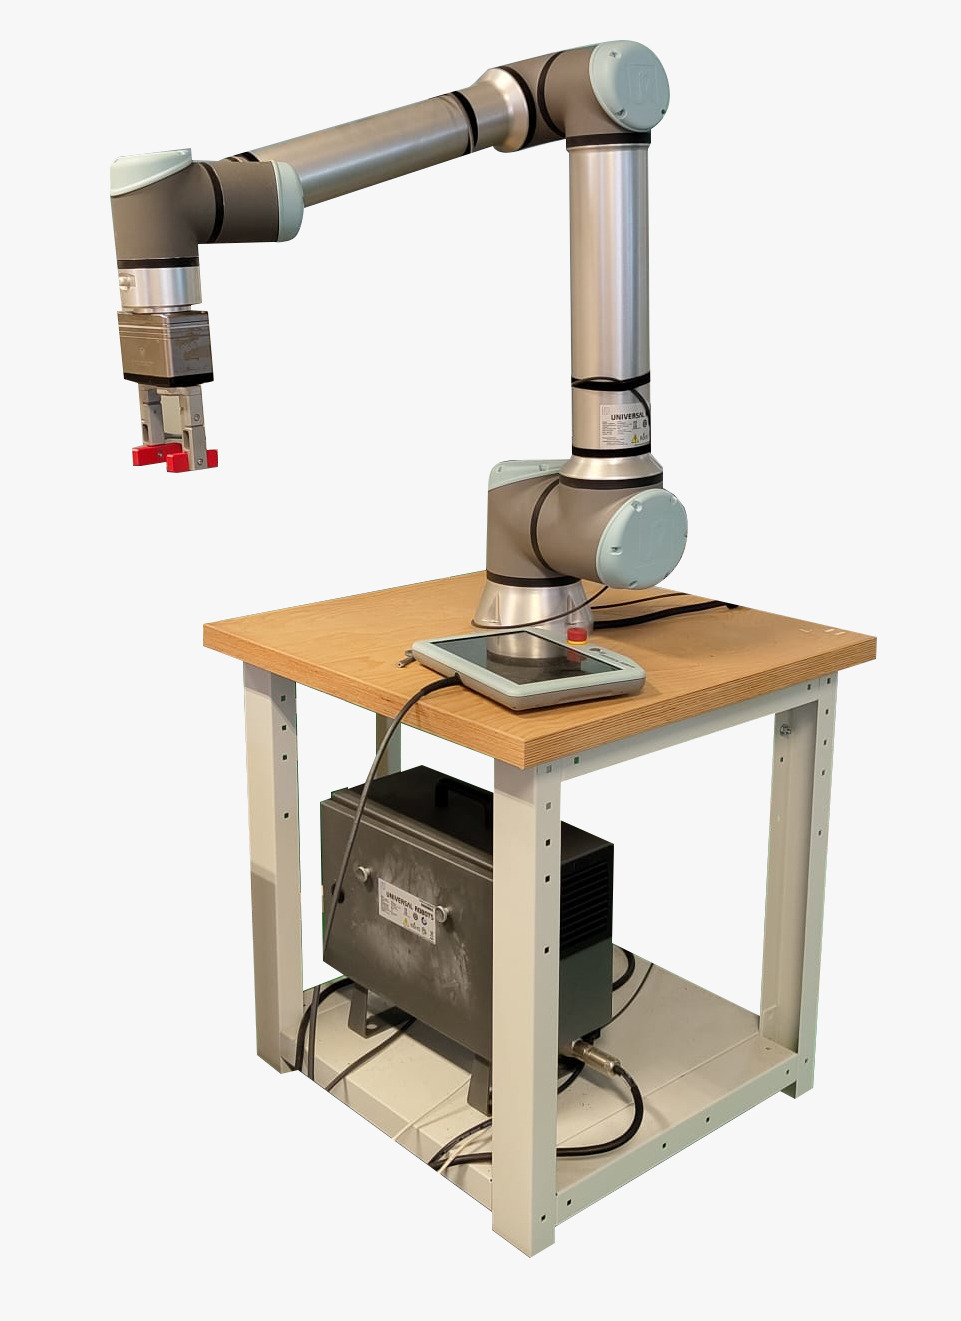
\includegraphics[width=0.4\linewidth]{figs/ur10e.jpeg}
    \caption{Robot UR10e used for the development of the dissertation work, available at IRIS-LAB, University of Aveiro}
    \label{f:ur10e_iris}
\end{figure}

\section{Marker Detection}
\label{section:marker-detection}
% 
% Vuforia is a software platform that enables the creation of \ac{ar} experiences. 
% % Integrated with Unity, a leading platform for developing games and interactive applications, Vuforia simplifies the incorporation 
% of AR into mobile and digital apps. 
% It uses computer vision technologies to recognize and track images and objects in the real world, allowing developers to overlay digital 
% content precisely.

% The marker illustrated in Figure \ref{f:aruco_marker} was selected following initial attempts that yielded inconsistent results when using 
% the laptop's camera, shown in the figure \ref{fig:camera-c922}, to scan the environment. This particular marker demonstrated greater stability, 
% enabling the precise positioning of the digital UR10 model in alignment with the physical surroundings. Consequently, this facilitated the accurate 
% overlay of the digital UR10 model onto the actual UR10e robot, enhancing the integration of virtual and real-world elements.

% \begin{figure}[h]
%     \centering
%       \begin{subfigure}[b]{0.45\textwidth}
%       \centering
%       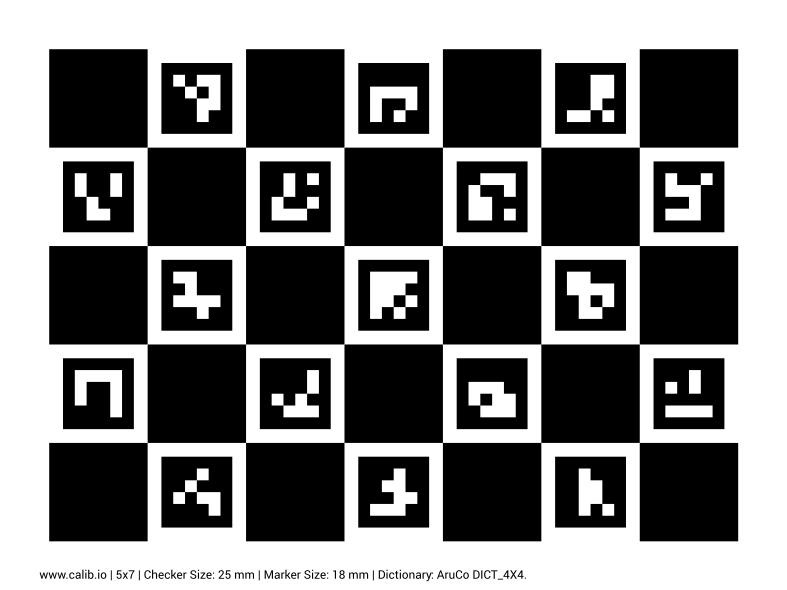
\includegraphics[width=0.7\textwidth]{figs/calib_io_charuco_200x150_5x7_25_18_DICT_4X4.png}
%       \caption{ArUco marker used to allow the segmentation for aligning the digital twin accordingly to the real environment}
%       \label{f:aruco_marker}
%       \end{subfigure}
%         \hfill % This command adds space between the subfigures
%       \begin{subfigure}[b]{0.45\textwidth}
%           \centering
%           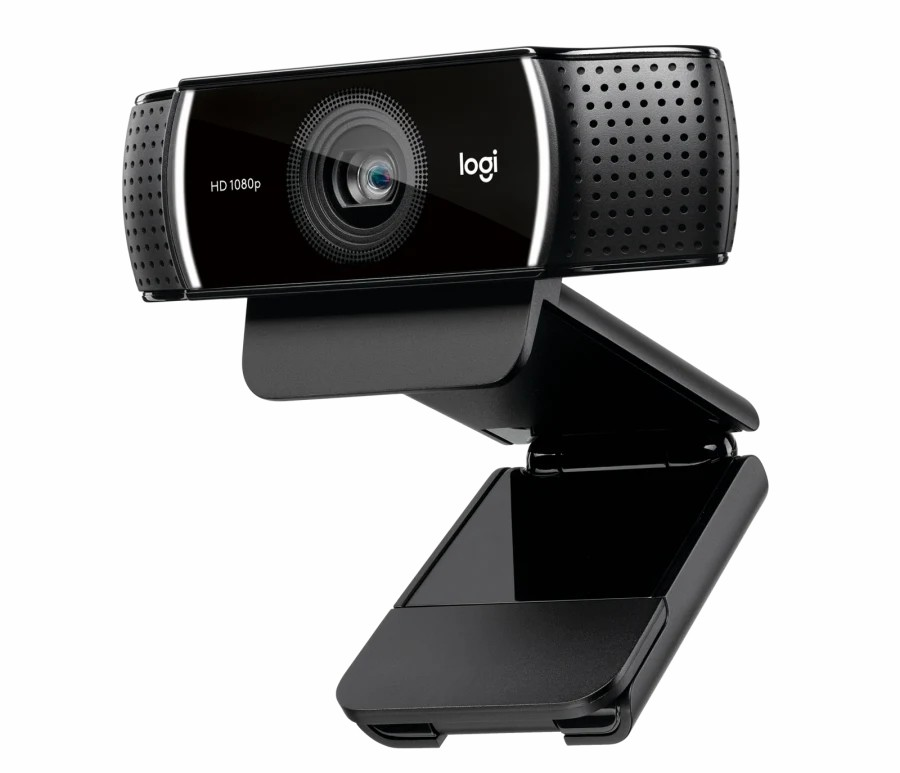
\includegraphics[width=0.7\linewidth]{figs/camera-c922.jpg}
%           \caption{Logitech c922 camera, used for testing on-site application developments}
%           \label{fig:camera-c922}
%       \end{subfigure}
%       \caption{ArUco marker used with the Logitech c922 camera for segmentation and manipulation of virtual environment}
%   \label{marker-camera}
%   \end{figure}
   commented this part because text is below - choose whether to use this or the text below


    Vuforia is a software platform that enables the creation of \ac{AR} experiences. 
    % Integrated with Unity, a leading platform for developing games and interactive applications, Vuforia simplifies the incorporation 
    of AR into mobile and digital apps. 
    It uses computer vision technologies to recognize and track images and objects in the real world, allowing developers to overlay digital 
    content precisely.

    The marker illustrated in Figure \ref{f:aruco_marker} was selected following initial attempts that yielded inconsistent results when using 
    the laptop's camera, shown in the figure \ref{fig:camera-c922}, to scan the environment. This particular marker demonstrated greater stability, 
    enabling the precise positioning of the digital UR10 model in alignment with the physical surroundings. Consequently, this facilitated the accurate 
    overlay of the digital UR10 model onto the actual UR10e robot, enhancing the integration of virtual and real-world elements.

    \begin{figure}[h]
        \centering
        \begin{subfigure}[b]{0.45\textwidth}
        \centering
        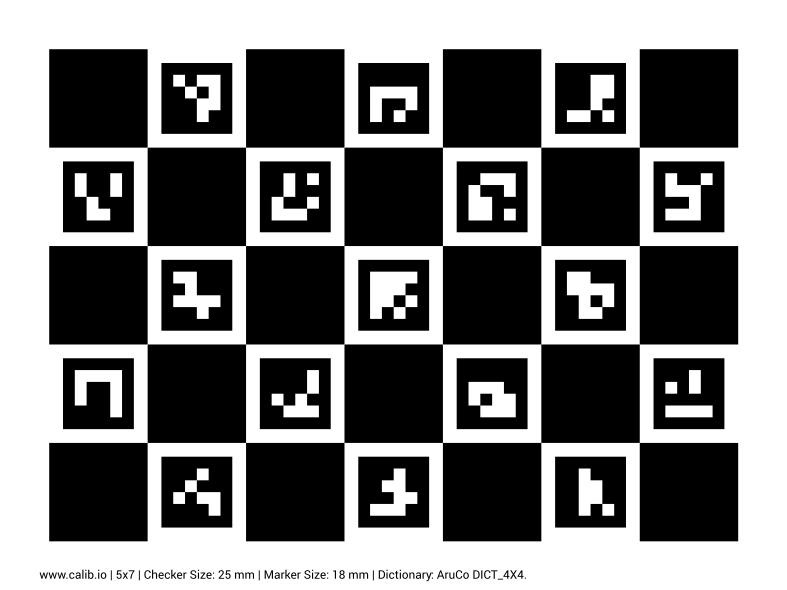
\includegraphics[width=0.7\textwidth]{figs/calib_io_charuco_200x150_5x7_25_18_DICT_4X4.png}
        \caption{ArUco marker used to allow the segmentation for aligning the digital twin accordingly to the real environment}
        \label{f:aruco_marker}
        \end{subfigure}
            \hfill % This command adds space between the subfigures
        \begin{subfigure}[b]{0.45\textwidth}
            \centering
            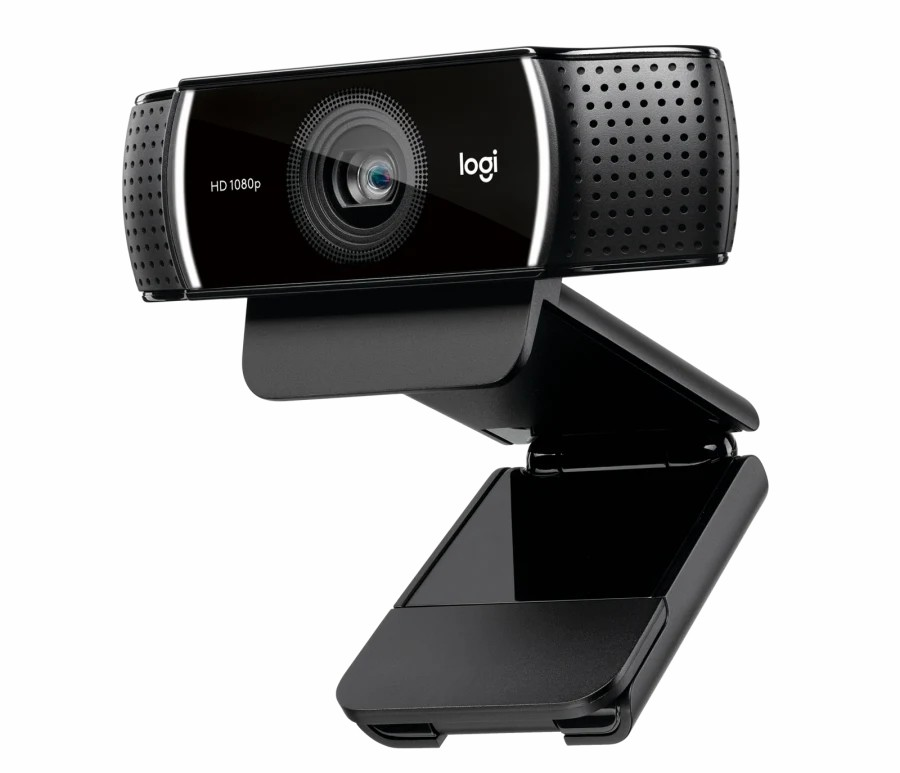
\includegraphics[width=0.7\linewidth]{figs/camera-c922.jpg}
            \caption{Logitech c922 camera, used for testing on-site application developments}
            \label{fig:camera-c922}
        \end{subfigure}
        \caption{ArUco marker used with the Logitech c922 camera for segmentation and manipulation of virtual environment}
    \label{marker-camera}
    \end{figure}
    
